\chapter{Electrical Networks}
This chapter focuses on electrical circuits, a particular type of network. \footnote{We will often refer to an electrical network as a circuit.} Not surprisingly, circuit models contain nodes (junctions) and edges (wires or other components). The edges have values associated with them. And, we'll see that these networks obey certain rules.\par

\section{Electrical Charge}
Similar to road networks and water networks, something flows on the edges of electrical networks: electric charge. Unfortunately, though, moving electric charge can be harder to picture than driving cars or the flow of water.\par

\vspace{6pt}
\setlength{\hangindent}{30pt}\noindent
\textbf{Good Question:} What, exactly, is electrical charge? \par
\vspace{6pt}
\setlength{\hangindent}{30pt}\noindent
\textbf{Non-fullfilling Answer:} It is a property that some particles have. \par
\vspace{6pt}
\setlength{\hangindent}{30pt}\noindent
\textbf{Good Question:} But what's it made of? \par
\vspace{6pt}
\setlength{\hangindent}{30pt}\noindent
\textbf{Non-fullfilling Answer:} Sorry, but it might not be helpful to think of it as made of anything - it is just a property, like being symmetrical. However, so far, all particles with charge also have mass. Furthermore, and maybe surprisingly (or not\footnote{If charge weren't quantized then it would take an infinite amount of information to describe just the amount of charge on one ion. That really would be an odd universe. Take your pick which seems more odd to you.}) it comes in discrete chunks. We'll write ($1 e^-$) as the charge on 1 electron.

\begin{blevel}
Fill in the rest of Table~\ref{T:2EP}. Look stuff up online as needed.
\end{blevel}

\par
\begin{table}[H]
\begin{center}
\begin{tabular}{|c|c|} \hline
particle	&	charge (units of $e^-$) \\ \hline
electron	&	-1\\ \hline
proton		&	\\ \hline
top quark	&	\\ \hline
muon		&	\\ \hline
neutron		&	\\ \hline
photon		&	\\ \hline
Sodium Ion	&	\\ \hline
\end{tabular}
\caption{Summary of amount of charge that some particles have}
\label{T:2EP}
\end{center}
\end{table}

\begin{alevel}
What are the S.I. units of electrical charge?
\end{alevel}

\begin{blevel}
How many electrons would add up to one Coulomb of charge?
\end{blevel}

\subsection{Electrical Current}
Charge flows along the edges of electrical networks. We measure this flow in units of charge per time and we call (a flowrate of one Coulomb per one second) an (Ampere or Amp). Of course, $\frac{1}{10}$ of a Coulomb per $\frac{1}{10}$ second, would also equal one Amp of current during that time interval.
\par
\begin{alevel}
A wire carries a current of 5 Amps. How many Coulombs of charge pass through the wire each second? Each minute?
\end{alevel}

\begin{blevel}
A wire carries a current of 5 Amps. How many electrons pass through the wire each second? Each minute?
\end{blevel}

\begin{blevel}
Fill in table~\ref{F:2SU}.
\end{blevel}

\par
\begin{table}[H]
\begin{center}
\begin{tabular}{|c|c|c|c|} \hline
item	&	abbreviation & units & units abbreviation \\ \hline
Force	&	F	& Newton	& N\\ \hline
	&		&	&	kg	\\ \hline
charge	& q	&&	\\ \hline
current		&&&	\\ \hline
temperature		&&&	\\ \hline
Energy	&&&	\\ \hline
Power	&&&	\\ \hline
\end{tabular}
\caption{Symbols and units}
\label{F:2SU}
\end{center}
\end{table}

\noindent
The relationship between current, charge and time mirrors the relationship between acceleration, velocity and time. Electric current is the instantanous rate at which charge passes along an edge, just like acceleration is the instantaneous rate at which velocity is changing. \footnote{If anything, it is simpler because we don't need to worry about current or charge being vectors, at least not in this context.} 

\par
\begin{align}
\vec{a} = \frac{d\vec{v}}{dt}&&\leftrightarrow&&I = \frac{dq}{dt}
\end{align}
\par
Figure~\ref{F:2CAR} shows the velocity of a car as a function of time.
\par
\begin{figure}[H]
\begin{center}
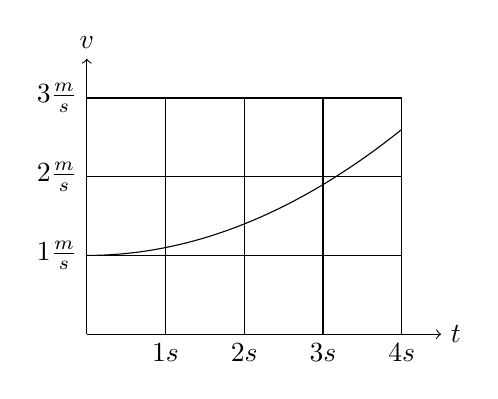
\begin{tikzpicture}
\draw[->] (0,0)--(4.5,0) node[right] {$t$};
\draw[->] (0,0)--(0,3.5) node[above] {$v$};
\draw (0,1)node[left] {$1 \frac{m}{s}$} --(4,1);
\draw (0,2)node[left] {$2 \frac{m}{s}$}--(4,2) ;
\draw (0,3)node[left] {$3 \frac{m}{s}$}--(4,3) ;
\draw (1,0)node[below] {$1 s$}--(1,3) ;
\draw (2,0)node[below] {$2 s$}--(2,3) ;
\draw (3,0)node[below] {$3 s$}--(3,3) ;
\draw (4,0)node[below] {$4 s$}--(4,3) ;
\draw [smooth, samples=100,domain=0:4] plot(\x,{.1*(\x)*(\x)+1});
\end{tikzpicture}
\caption{A car's velocity as a function of time.}
\label{F:2CAR}
\end{center}
\end{figure}

\begin{alevel}
How fast is the car going at 4 seconds?
\end{alevel}

\begin{blevel}
Trick question: What is the position of the car after 1 s?
\end{blevel}

\begin{dlevel}
Why was the previous question a trick question? What piece of information was missing?
\end{dlevel}

\begin{blevel}
What is the average acceleration of the car between 0 and 4 seconds?
\end{blevel}

\begin{blevel}
What is the instantaneous acceleration of the car when the time is 0 seconds? Hint: acceleration is the slope of a v-t graph.
\end{blevel}

\begin{blevel}
What is the instantaneous acceleration of the car at a time of 4 seconds?
\end{blevel}
\begin{clevel}
Sketch the car's acceleration between t=0 and t=4 s. Label your axes.
\end{clevel}
\noindent
Consider the graph in Figure~\ref{F:2QT} which shows the charge at some node as a function of time.
\par
\begin{figure}[H]
\begin{center}
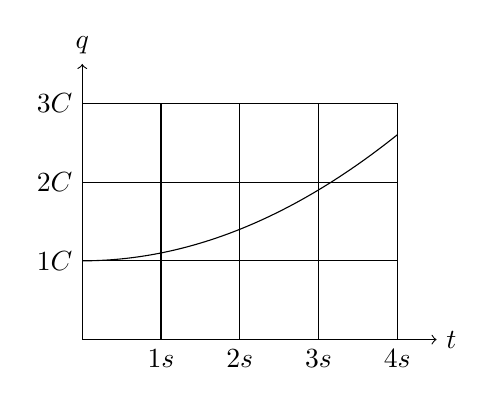
\begin{tikzpicture}
\draw[->] (0,0)--(4.5,0) node[right] {$t$};
\draw[->] (0,0)--(0,3.5) node[above] {$q$};
\draw (0,1)node[left] {$1 C$} --(4,1);
\draw (0,2)node[left] {$2 C$}--(4,2) ;
\draw (0,3)node[left] {$3 C$}--(4,3) ;
\draw (1,0)node[below] {$1 s$}--(1,3) ;
\draw (2,0)node[below] {$2 s$}--(2,3) ;
\draw (3,0)node[below] {$3 s$}--(3,3) ;
\draw (4,0)node[below] {$4 s$}--(4,3) ;
\draw [smooth, samples=100,domain=0:4] plot(\x,{.1*(\x)*(\x)+1});
\end{tikzpicture}
\caption{Charge as a function of time.}
\label{F:2QT}
\end{center}
\end{figure}

\begin{alevel}
How much charge is on the node after 4 seconds?
\end{alevel}
\begin{blevel}
What is the average current into the node between 0 and 4 seconds?
\end{blevel}
\begin{blevel}
What is the instantaneous current into the node at a time of 4 seconds?
\end{blevel}
\begin{clevel}
Graph the current into the node, I(t), between t=0 and t=4 s.
\end{clevel}

\begin{alevel}
A node has a net current entering it of $i=(3q+1)$ Amps. What are the units of the '3'?
\end{alevel}

\begin{clevel}
A node has a net current entering it of $i=(3q+1)$ Amps. The initial amount of charge at the node  is 5 C. Determine the amount of charge present at the node as a function of time.
\end{clevel}

\begin{clevel}
A node has a net charge on it of $q=(3e^{2t}+1)$ Coulombs. Determine the current onto this node as a function of time.
\end{clevel}

%%%%%%%%%%%%%%%%%%%%%%%%%%%%%%%%%%%%%%%%%%%%%%%%%%%%%%%%%
\section{Voltage}
Like electrical current, voltage is also a special quantity in analyzing electrical networks. This section deals with learning what voltage is and how it might be useful.\par

A voltage difference represents an electrical energy difference per amount of charge. That takes a little time to unpack. Let's start with reviewing what we mean by energy.

\subsection{Energy}
We need energy to do anything. An object that speeds up gains kinetic energy. It takes work (a transfer of energy) to drag something across the floor. It takes energy to create mass and, likewise, mass can be converted back into energy (atomic bombs). In this class, we are particularly concerned with the electrical energy needed to squish charges together.
\par
\begin{clevel}
Fill in the rest of this table. Look up formulae as needed.
\end{clevel}

\begin{table}[H]
\begin{center}
\begin{tabular}{|c| c| c|} \hline
item & relevant formula	& rough value \\ \hline
stand up	& W = F*d	& $(100kg)*(9.8 \frac{m}{s^2})*.5 m \approx 500J$\\ \hline
heat up cup of coffee &	& \\ \hline
start running sideways	&	&\\ \hline
drag a log 20 feet	&	&\\ \hline
create a 1kg of mass	&	&\\ \hline
create one photon ($\lambda$=650 nm)	&	&	\\ \hline
case A*			&	&\\ \hline
case B*			&	&\\ \hline
\end{tabular}
\caption{Approximate amount of energy needed to do several tasks.}
\end{center}
\end{table}

\noindent
*case A: Move two electrons from a distance of 4 m apart to a distance of 2 m apart.
\par
\noindent
*case B: Separate two 1kg masses that are initially 2m apart to make them 4 m apart\footnote{The gravitational potential energy is for the system, not just one of the masses by itself}.
\linebreak

\begin{blevel}
What is the principle of conservation of energy?
\end{blevel}

\par
To understand voltage, it might be useful to begin by studying its gravitational counterpart, gravitational potential energy per mass. Figure~\ref{F:2MT} shows a mountain with a hiking trail network starting at the parking lot labeled P:
\par
\begin{figure}[H]
\begin{center}
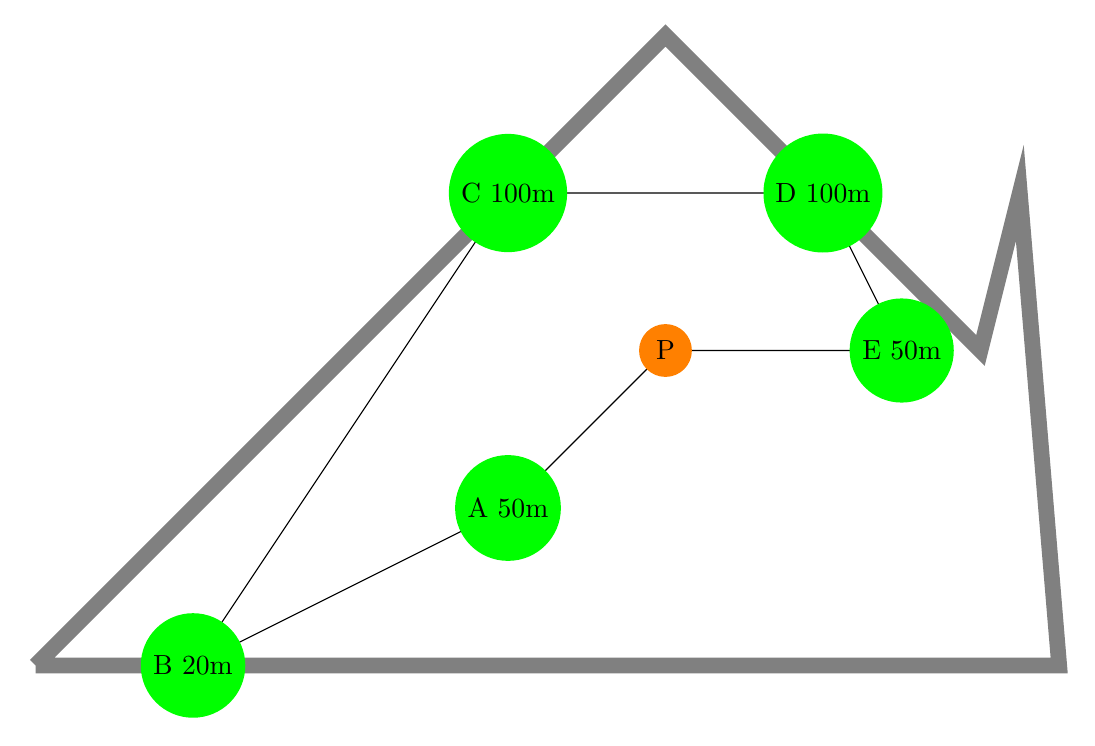
\begin{tikzpicture}
\draw [draw=gray, line width=2mm] (0,0)--(8,8)--(12,4)--(12.5,6)--(13,0)--(0,0);
\draw (8,4) node[circle, radius=0.25cm, fill=orange] {P}
--(6,2) node[circle, radius=0.25cm, fill=green] {A 50m}
--(2,0) node[circle, radius=0.25cm, fill=green] {B 20m}
--(6,6) node[circle, radius=0.25cm, fill=green] {C 100m}
--(10,6) node[circle, radius=0.25cm, fill=green] {D 100m}
--(11,4) node[circle, radius=0.25cm, fill=green] {E 50m} -- cycle;
\end{tikzpicture}
\caption{A mountain with a parking lot, P and a trail system. The labels indicate the heights of those points above some reference point.}
\label{F:2MT}
\end{center}
\end{figure}

\begin{alevel}
What do the edges in the network represent?
\end{alevel}
\begin{blevel}
Do the nodes in the network have a number associated with them? What is it?
\end{blevel}
\begin{alevel}
What is the total change in height when hiking from the parking lot, around the trail, and back to the parking lot?
\end{alevel}
\begin{blevel}
Generalize your answer to the above question.
\end{blevel}
\begin{blevel}
Suppose a 50 kg hiker named Comet and an 80kg hiker named Ajax start at the parking lot and hike to point D. What are the respective changes in gravitational potential energy for the Comet-Earth system and the Ajax-Earth system? What are the corresponding gains in gravitational potential energy per mass?
\end{blevel}

Tracking changes in (gravitational potential energy per mass) can be useful because these changes only depend on the shape of the trail, not who is hiking it. Scientists shorten (gravitational potential energy per mass) to (gravitational potential) and give it the symbol V (I'll use $V_G$ so as not to confuse it with Voltage, V).
\begin{align}
V_G=\frac{PE_{GRAV}}{m}&&\text{Gravitational Potential} \label{E:2GP}
\end{align}

Let's write the gravitational potential difference from A to B as $V_{AB}$. If pt. B represents a higher grav. potential than A, this would be positive. Note that: $V_{AB}=-V_{BA}$.

\begin{blevel}
Use the above mountain trail graphic to fill in Table~\ref{T:2GP}.
\end{blevel}

\begin{table}[H]
\begin{center}
\begin{tabular}{|c|c|}\hline
pts&Grav. Potential ($V_G$)\\ \hline
$V_{AB}$& \\ \hline
$V_{AC}$& \\ \hline
$V_{CE}$& \\ \hline
$V_{CD}$& \\ \hline
$V_{EC}$& \\ \hline
\end{tabular}
\caption{Values for gravitational potential energy per mass (gravitational potential)}
\label{T:2GP}
\end{center}
\end{table}

\begin{clevel}
Does gravitation potential flow?
\end{clevel}

\begin{blevel}
What are the units of gravitational potential?
\end{blevel}

\subsection{Voltage - finally}
Instead of gravitational energy per mass, we'll be using its electrical equivalent, electrical energy per charge. Some people call it the electric potential, but in the context of electrical networks, we usually say Voltage. \par

Consider Figure~\ref{F:2Va}. If it takes 5 Joules of energy to move +2 Coulombs of charge from pt A to pt B, then we would say there is a 2.5 Volt difference between pts A and B.

\begin{figure}[H]
\begin{center}
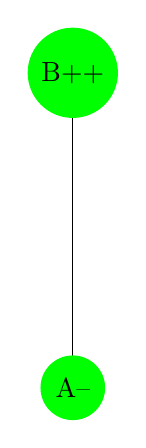
\begin{tikzpicture}
\draw (2,0) node[circle, radius=0.25cm, fill=green] {A--}
--(2,4) node[circle, radius=0.25cm, fill=green] {B++};
\end{tikzpicture}
\caption{Two nodes. A has some negative charge and B has some positive charge.}
\label{F:2Va}
\end{center}
\end{figure}

The reason it would require energy (effort) to move charge from A to B is because B is positively charged, and the +2C charge would repel node B.
\par
\begin{blevel}
How much energy would it take to move 9C of charge from A to B?
\end{blevel}

\begin{alevel}
Does voltage flow?
\end{alevel}

\begin{blevel}
What is the electrical equivalent for Equation~\eqref{E:2GP}?
\end{blevel}

%%%%%%%%%%%%%%%%%%%%%%%%%%%%%%%%%
\subsection{Power}
Power is the rate at which energy is being transformed from one form to another. We (even scientists) might say consumed or produced, but we don't really mean it. The total enery in a closed system stays the same. You can't \emph{use up} energy. We're not producing energy, but rather transforming it from one form to another. The sun does not produce energy, it transforms it from mass energy into photons.
\par
\begin{alevel}
Does a power plant actually produce energy?
\end{alevel}

\begin{alevel}
(Energy per gallon) times (gallons per second). What units does this give?
\end{alevel}

\begin{blevel}
A 300W blender is in use for 25 seconds. How much energy does this use?
\end{blevel}

\begin{clevel}
A car gets 25 mpg. It travels 50 miles at a speed of 60 mph. At what rate (in Watts) is the car using its gas? Hint: How much time did it take to go 60 miles?
\end{clevel}

\begin{alevel}
How many Watts are equivalent to 1 horsepower?
\end{alevel}

\noindent\fbox{\parbox{\textwidth}{
\textbf{Example Power Calculation:}\par
Suppose water flows over a 4-meter tall water-wheel at a rate of 10 gallons per second. Estimate the rate at which the water wheel system can \emph{produce}\footnote{Again, we're really just transforming it from one form to another} power (assuming 100\% efficiency). Let's break this problem into a couple steps.

\par
\begin{itemize}
\item \textbf{Step 1:} Determine the gravitational potential energy difference per gallon of water. It will be the gravitational potential energy difference of the gallon being at the top of the water wheel verses at the bottom. Gravitional potential energy is mgh, or:
\begin{align*}
PE&=mgh\\
PE &= \rho (Volume)gh\\
\frac{PE}{V}&=\rho gh &\leftarrow&\text{potential energy per volume}\\
\frac{PE}{V}&= 1000*9.8*4 \approx 40000 \frac{J}{m^3}
\end{align*} 

Just convert this to gallons and we're done with this part.
\item \textbf{Step 2:} Recall that power is energy per time. We know energy per gallon. To convert to energy per time (power), multiply energy per gallon by gallons per second (given).
\end{itemize}

\begin{blevel}
What is the difference in $V_G$ between the bottom and top of the water wheel?
\end{blevel}

\begin{blevel}
Finish the above water wheel problem with the numbers given. Determine the power produced by the water wheel.
\end{blevel}

}}


\begin{blevel}
Justify the equation P=IV based on units. Hint: What are the units of current? What are the units of voltage (don't say Volts)?
\end{blevel}

\begin{clevel}
A well pump pushes water up from a depth of 200 feet. How much power is needed (in Watts) if the pump is to pump 10 gallons/minute?
\end{clevel}

\begin{clevel}
A 1000 kg car drives up a $5^0$ hill at 5 m/s. Ignore air drag. Determine the power needed from the engine.
\end{clevel}

\begin{blevel}
A resistor has a voltage difference across it of 5V and a current through it of 6Amps. How many Joules of energy does it dissipate each minute?
\end{blevel}

%%%%%%%%%%%%%%%%%%%%%%%%%%%%%%%%%%%%%%%%%%%%%%%%%%%%%%%%%%

\subsection{Application: Solar Cells}
Sunlight, like all light, is made of lots of individual packets of light called photons. Photons are interesting little particles in their own right. \footnote{For one thing, because they travel at the speed of light, time does not pass for a photon from its point of view. A photon is created and absorbed, potentially on the other side of the universe, at the same instant.}\par

Each photon transfers a small chunk of energy. Depending on how many photons are being absorbed and how much enery each one has, one can determine how much power is being transferred by light. At the Earth's surface, sunlight transfers about $1000 \frac{W}{m^2}$. Modern solar cells can capture about a quarter of this power.

A typical solar panel might produce 300 Watts in full sun\footnote{In 2021}.

\begin{alevel}
What is a particle of light called?
\end{alevel}
\begin{blevel}
How big (area) would a 300W solar panel need to be if it were 19\% efficient?
\end{blevel}
\begin{blevel}
If this panel were left out in the sun for 3 hours, how much energy would it collect?
\end{blevel}
\begin{blevel}
If this panel produced 48V, and were connected to a load designed to draw max power, how much current would it produce (still in full sun)?
\end{blevel}
\begin{blevel}
How many of these panels would be needed to generate 150 hp?
\end{blevel}

Consider the following two arrangements of ways to connect two solar panels. In both cases the individual panels produce 300W at a voltage of 48V.
\par

\begin{figure}[H]
\begin{center}
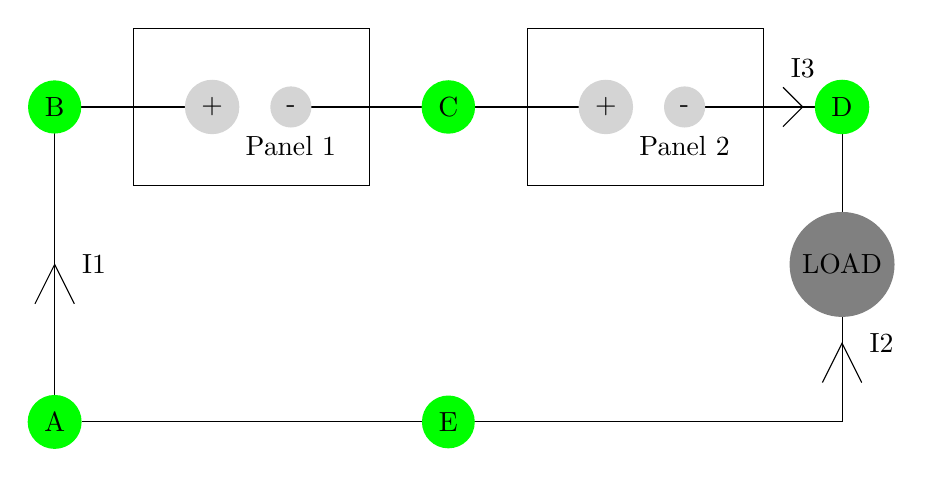
\begin{tikzpicture}
\draw (0,0) node[circle, radius=0.25cm, fill=green] (A) {A}
--(0,4) node[circle, radius=0.25cm, fill=green] {B}
--(2,4) node[circle, radius=0.1cm, fill={rgb:black,1;white,5}] {+};
\draw (3,4) node[circle, radius=0.1cm, fill={rgb:black,1;white,5}] {-}
--(5,4) node[circle, radius=0.25cm, fill=green] {C}
--(7,4) node[circle, radius=0.1cm, fill={rgb:black,1;white,5}] {+};
\draw (8,4) node[circle, radius=0.1cm, fill={rgb:black,1;white,5}] {-}
--(10,4) node[circle, radius=0.25cm, fill=green] {D}
--(10,2) node[circle, radius=0.1cm, fill={rgb:black,1;white,1}] {LOAD}
--(10,0)
--(5,0) node[circle, radius=0.25cm, fill=green] {E}
--(A);
\draw [draw=black] (1,3) rectangle (4,5);
\draw [draw=black] (6,3) rectangle (9,5);
\node at (3,3.5) {Panel 1};
\node at (8,3.5) {Panel 2};
\draw (-.25,1.5)--(0,2)--(.25,1.5) (.5,2) node{I1};
\draw (9.75,.5)--(10,1)--(10.25,.5) (10.5,1) node{I2};
\draw (9.25,3.75)--(9.5,4)--(9.25,4.25) (9.5,4.5) node{I3};
\end{tikzpicture}
\caption{Arrangment 1.}
\end{center}
\end{figure}

\begin{figure}[H]
\begin{center}
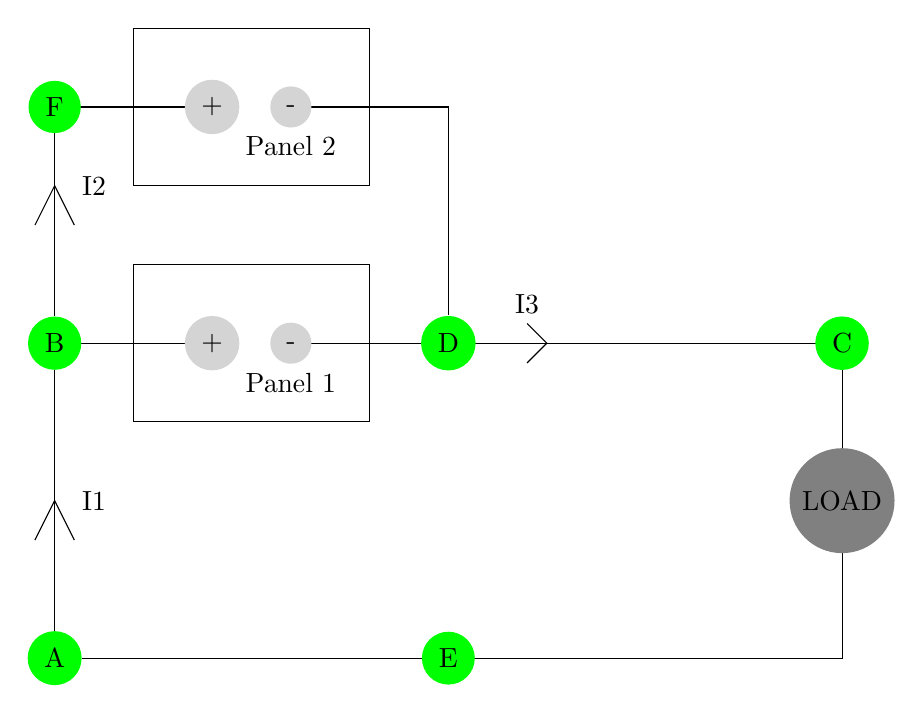
\begin{tikzpicture}
\draw (0,0) node[circle, radius=0.25cm, fill=green] (A) {A}
--(0,4) node[circle, radius=0.25cm, fill=green] (B) {B}
--(2,4) node[circle, radius=0.1cm, fill={rgb:black,1;white,5}] {+}
(3,4) node[circle, radius=0.1cm, fill={rgb:black,1;white,5}] {-}
--(5,4) node[circle, radius=0.25cm, fill=green] (D) {D}
--(10,4) node[circle, radius=0.25cm, fill=green] {C}
--(10,2) node[circle, radius=0.1cm, fill={rgb:black,1;white,1}] {LOAD}
--(10,0)
--(5,0) node[circle, radius=0.25cm, fill=green] {E}
--(A);
\draw (B)--(0,7) node[circle, radius=0.25cm, fill=green] {F}
--(2,7) node[circle, radius=0.1cm, fill={rgb:black,1;white,5}] {+}
(3,7) node[circle, radius=0.1cm, fill={rgb:black,1;white,5}] {-}
--(5,7)--(D);
\draw [draw=black] (1,3) rectangle (4,5);
\draw [draw=black] (1,6) rectangle (4,8);
\node at (3,3.5) {Panel 1};
\node at (3,6.5) {Panel 2};
\draw (-.25,1.5)--(0,2)--(.25,1.5) (.5,2) node{I1};
\draw (-.25,5.5)--(0,6)--(.25,5.5) (.5,6) node{I2};
\draw (6,3.75)--(6.25,4)--(6,4.25) (6,4.5) node{I3};
\end{tikzpicture}
\caption{Arrangment 2.}
\end{center}
\end{figure}

\begin{blevel}
Fill in the following table.
\end{blevel}
\par
\begin{table}[H]
\begin{center}
\begin{tabular}{|c|c|c|}\hline
which points	& Voltage (Arrangement 1)&Voltage (Arrangement 2) \\ \hline
BC & & \\ \hline
CB & & \\ \hline
AB & & \\ \hline
BD & & \\ \hline
DE & & \\ \hline
DA & & \\ \hline
AD & & \\ \hline
FD & n/a & \\ \hline	
\end{tabular}
\end{center}
\end{table}

\begin{blevel}
For any arrangement, how much current must be flowing through Panel 1 and Panel 2 in order for them to each produce 300W of power? Note: Since the panel is producing power, the current would flow from the negative side to the positive side.
\end{blevel}

Note the arrows labeled on some of the wires. These arrows indicate the current passing through those wires.
\par
\begin{blevel}
Fill in the currents indicated in Table~\ref{T:2SSC}.
\end{blevel}

\par
\begin{table}[H]
\begin{center}
\begin{tabular}{|c|c|c|}\hline
which current	& Current (Arrangement 1)&Current (Arrangement 2) \\ \hline
I1 & & \\ \hline
I2 & & \\ \hline
I3 & & \\ \hline
\end{tabular}
\label{T:2SSC}
\end{center}
\end{table}

\begin{blevel}
Determine the voltage difference across the load and the current through the load for both arrangements. For each case, calculate the power absorbed by the load.
\end{blevel}

\begin{clevel}
Design, using 100W, 20V panels an arrangment of panels that produces 40V at the load and 800W of power.
\end{clevel}

%%%%%%%%%%%%%%%%%%%%%%%%%%%%%%%%%%%%%%%%%%%%%%%%%%%%%%%%%%%
\subsection{Application: Electric cars}
Electric cars store energy and convert that energy into motion when you drive.\par

A gallon of gas stores about 100 Million Joules of energy. (Great Scott! That's a lot of energy.) Diesel fuel stores a little more energy per gallon than regular unleaded gas. Electric cars store the energy in a electrical battery\footnote{How the energy is stored isn't really what makes it an electric car. A fun conversation could be had on what exactly an electric car needs to have in order to be called an electric car.}. Alternatively, one could store the energy as gas, then use it to charge a battery, then use the battery to power the motor\footnote{It's up to you as whether or not you'd still call it an electric car}.

\begin{figure}[H]
\begin{center}
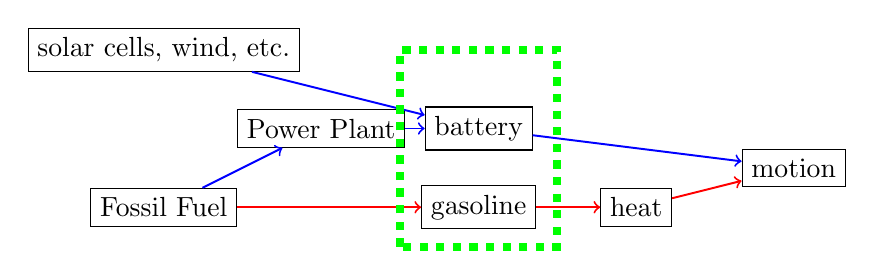
\begin{tikzpicture}
\draw (0,0) node[draw=black, radius=.25 cm, fill=white](G){gasoline}
(2,0) node[draw=black, radius=.25 cm, fill=white](H){heat}
(4,.5) node[draw=black, radius=.25 cm, fill=white](M){motion};
\draw [draw=red, line width=0.25mm] [->] (G)--(H);
\draw [draw=red, line width=0.25mm] [->] (H)--(M);
\draw (-2,1) node[draw=black, radius=.25 cm, fill=white](PP){Power Plant}
(-4,2) node[draw=black, radius=.25 cm, fill=white](SS){solar cells, wind, etc.}
(0,1) node[draw=black, radius=.25 cm, fill=white](B){battery}
(-4,0) node[draw=black, radius=.25 cm, fill=white](FF){Fossil Fuel};
\draw [draw=blue, line width=0.25mm] [->] (B)--(M);
\draw [draw=blue, line width=0.25mm] [->] (SS)--(B);
\draw [draw=blue, line width=0.25mm] [->] (PP)--(B);
\draw [draw=red, line width=0.25mm] [->] (FF)--(G);
\draw [draw=blue, line width=0.25mm] [->] (FF)--(PP);
\draw [draw=green, line width=1 mm, dashed] (-1,-.5)--(-1,2)--(1,2)--(1,-.5)--(-1,-.5);
\end{tikzpicture}
\caption{Energy transfer chains for electric cars (blue) and gas cars (red). The dashed box represents the energy storage options for the car.}
\end{center}
\end{figure}

We quantify the amount of amount of energy stored in a battery with a variety of units. One could certainly use Joules, but many times people use a common alternative called the kilo-Watt-hour. One kWr stores the equivalent amount of energy as using 1000 Watts for one hour.

\begin{alevel}
If someone uses 10 Watts for 20 seconds, how much energy did they use?
\end{alevel}

\begin{blevel}
Someone says they have a solar panel that produces 500W per day. Why is this a confusing statement?
\end{blevel}

\begin{blevel}
How many Joules are equivalent to 1 kW-hr?
\end{blevel}

\begin{blevel}
A 300W solar panel sits out in direct sun for 5 hours. How many kWhr of energy does it collect?
\end{blevel}

\begin{blevel}
How many kWhr are equivalent to 1 gallon of gas? \footnote{This is a little misleading because the gas will be burned to produce thermal energy and then that thermal energy is transformed into kinetic energy. The process is less efficient than the direct conversion of chemical potential energy stored in a battery into the motion of the car. In order words, at least for cars, 1 kWhr or battery storage is more valuable than 1 kWhr of gas.}
\end{blevel}

When buying electricity through the grid, you will probably pay per kWhr, the cost of which is around 20 cents in NY (year 2021)\footnote{Delivered, including transport costs, not just generation}.

\begin{blevel}
The 2021 Chevvy Bolt has a battery size of 65kWhrs. How many Joules does this battery store? If someone comes to your house and needs to charge their entire car battery through your garage plug, how much will this cost you? 
\end{blevel}

\begin{blevel}
You plug your electric car into a normal wall outlet to charge up. The wall outlet can not draw more than 10A without tripping a breaker and has a voltage of 120V. Determine the max power that can be drawn from the outlet to charge the car. At this max power, how much time will it take to charge the car battery? Assume the battery starts as a dead battery. 
\end{blevel}

\begin{blevel}
Special chargers have been constructed that can draw much more power than your wall outlet can provide. These chargers can deliver more like 200,000 Watts. How much time will these super chargers take to charge up an electric car like the Chevvy Bolt?
\end{blevel}


%%%%%%%%%%%%%%%%%%%%%%%%%%%%%%%%%%%%%%%%%%%%%%%%%%%%%%%%%%%
\section{Network Summary Table}

\begin{blevel}
Fill in this table.
\end{blevel}

\par
\begin{table}[H]
\begin{center}
\begin{tabular}{ |c | c | c | c |} \hline
network	&	what are nodes	& what are edges	& what flows \\ \hline
friends	&	people	& indications of friendship	& n/a \\ \hline
traffic &		&				&	\\ \hline
water	&		&				&	\\ \hline
electrical	& places of equal electrical energy	&	&	\\ \hline
\end{tabular}
\caption{Network Summary Table}
\end{center}
\end{table}

%%%%%%%%%%%%%%%%%%%%%%%%%%%%%%%%%%%%%%%%%%%%%%%%%%%%%%%%%%%%%%%%%%%%%%%%%%%%%%%%%
\section{An Important Summary Diagram: The Six Circles.}
This chapter covered some of quantities relevant to electrical networks, like energy, voltage, charge, and current. Eventually, you may also need to keep straight electric fields, gravitational fields, forces and work. Table~\ref{F:26C} summarizes the relationships between some of these parameters and may help place voltage and force in a larger context.
\par
Start with the relationship between force and potential energy. Dividing these quantities by mass results in the gravitational field and gravitational potential. Divide by charge instead leads to electric field and voltage. Use the same relationships to move left-right or uo-down on the diagram. Knowing these relationships means you actually know all 14 equations!
\par
\begin{figure}[H]
\begin{center}
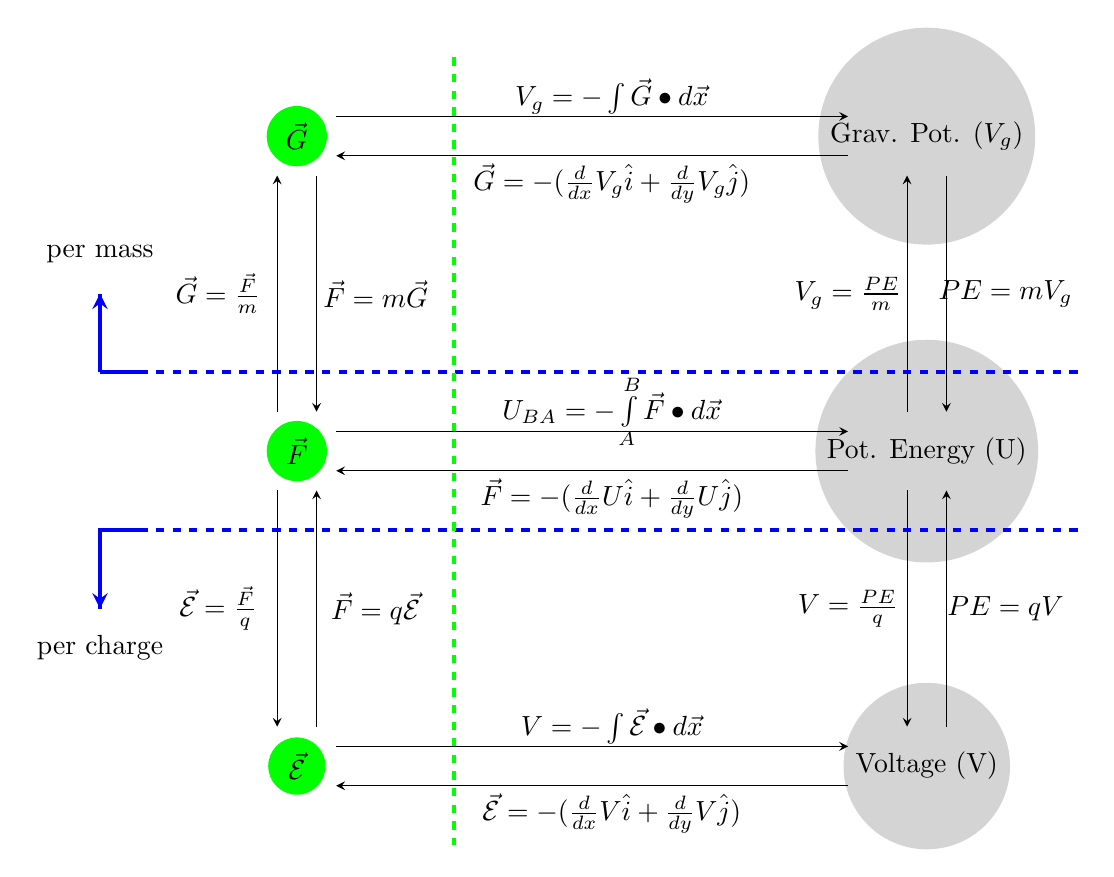
\begin{tikzpicture}
\draw (0,0) node[circle, radius=0.25cm, fill=green] (F) {$\vec{F}$}
(0,4) node[circle, radius=0.25cm, fill=green] (G) {$\vec{G}$}
(8,4) node[circle, radius=0.25cm, fill={rgb:black,1;white,5}] {Grav. Pot. ($V_g$)}
(8,0) node[circle, radius=0.1cm, fill={rgb:black,1;white,5}] (E) {Pot. Energy (U)}
(0,-4) node[circle, radius=0.25cm, fill=green] (Ef) {$\vec{\mathcal{E}}$}
(8,-4) node[circle, radius=0.25cm, fill={rgb:black,1;white,5}] {Voltage (V)};
%vertical
\draw [-stealth](-.25,.5)--(-.25,3.5);
\draw [stealth-](.25,.5)--(.25,3.5);
\draw node at (-1,2) {$\vec{G} = \frac{\vec{F}}{m}$};
\draw node at (1,2) {$\vec{F} = m\vec{G}$};
\draw [-stealth](7.75,.5)--(7.75,3.5);
\draw [stealth-](8.25,.5)--(8.25,3.5);
\draw node at (7,2) {$V_g = \frac{PE}{m}$};
\draw node at (9,2) {$PE = mV_g$};
\draw [-stealth](-.25,-.5)--(-.25,-3.5);
\draw [stealth-](.25,-.5)--(.25,-3.5);
\draw node at (-1,-2) {$\vec{\mathcal{E}} = \frac{\vec{F}}{q}$};
\draw node at (1,-2) {$\vec{F} = q\vec{\mathcal{E}}$};
\draw [-stealth](7.75,-.5)--(7.75,-3.5);
\draw [stealth-](8.25,-.5)--(8.25,-3.5);
\draw node at (7,-2) {$V = \frac{PE}{q}$};
\draw node at (9,-2) {$PE = qV$};
%horizontal
\draw [-stealth] (.5,.25)--(7,.25);
\draw [stealth-] (.5,-.25)--(7,-.25);
\draw node at (4,.5) {$U_{BA} = -\int\limits_A^B{\vec{F}\bullet d\vec{x}}$};
\draw node at (4,-.6) {$\vec{F} = -(\frac{d}{dx}U\hat{i}+\frac{d}{dy}U\hat{j})$};
\draw [-stealth] (.5,4.25)--(7,4.25);
\draw [stealth-] (.5,3.75)--(7,3.75);
\draw node at (4,4.5) {$V_g = -\int{\vec{G}\bullet d\vec{x}}$};
\draw node at (4,3.4) {$\vec{G} = -(\frac{d}{dx}V_g\hat{i}+\frac{d}{dy}V_g\hat{j})$};
\draw [-stealth] (.5,-3.75)--(7,-3.75);
\draw [stealth-] (.5,-4.25)--(7,-4.25);
\draw node at (4,-3.5) {$V = -\int{\vec{\mathcal{E}}\bullet d\vec{x}}$};
\draw node at (4,-4.6) {$\vec{\mathcal{E}} = -(\frac{d}{dx}V\hat{i}+\frac{d}{dy}V\hat{j})$};
%
\draw [dashed, draw=blue,line width= 0.5mm] (-2,1) -- (10,1);
\draw [dashed, draw=blue,line width= 0.5mm] (-2,-1) -- (10,-1);
\draw [dashed, draw=green, line width= 0.5mm] (2,5) -- (2,-5);
\draw [draw=blue,line width= 0.5mm] (-2,1)--(-2.5,1)[stealth-](-2.5,2);
\draw [draw=blue,line width= 0.5mm] (-2.5,1)--(-2.5,2);
\draw node at (-2.5,2.5) {per mass};

\draw [draw=blue,line width= 0.5mm] [-stealth](-2.5,-1)--(-2.5,-2);
\draw [draw=blue,line width= 0.5mm] (-2,-1)--(-2.5,-1)--(-2.5,-2);
\draw node at (-2.5,-2.5) {per charge};
\end{tikzpicture}\\
\caption{The Six Circles}
\label{F:26C}
\end{center}
\end{figure}

\begin{alevel}
Based on the formulae on the diagram, identify two different units for voltage, other than Volts.
\end{alevel}

\begin{alevel}
Identify two different units for gravitational potential.
\end{alevel}

\begin{blevel}
The gravitational field at a point is $(10 N/kg) \hat{j}$. The electric field at that same point is $(-5 N/C) \hat{i}$. A 3 kg uncharged particle is placed there. What is the force acting on it? What is its acceleration?
\end{blevel}

\begin{blevel}
The gravitational field at a point is $(10 N/kg) \hat{j}$. The electric field at that same point is $(-5 N/C) \hat{i}$. A 3 kg particle with a charge of +2C is placed there. What is the magnitude of the net force acting on it? What is the magnitude of its acceleration?
\end{blevel}

\begin{blevel}
The gravitational field between points (0,0) and (1,0)m is $\vec{G}=(3x \frac{N}{kg})\hat{i}$. Is the gravitational potential higher at (1,0) or at (0,0)?
\end{blevel}

\begin{clevel}
The gravitational field between points (0,0) and (1,0)m is $\vec{G}=(3x \frac{N}{kg})\hat{i}$. How much energy would it take to move a 10 kg particle from (1,0) to (0,0)?
\end{clevel}

\begin{clevel}
The gravitational field between points (0,0) and (1,0)m is $\vec{G}=3x \frac{N}{kg}\hat{i}$. What is the $V_g$ difference between (1,0) to (0,0)?
\end{clevel}

\begin{clevel}
The electric field between points (0,0) and (2,0)m is $\vec{\mathcal{E}}=(5x+2)\hat{i} \frac{N}{C}$. What is the Voltage difference between (2,0) to (0,0)?
\end{clevel}

%%%%%%%%%%%%%%%%%%%%%%%%%%%%%%%%%%%%%%%%%%%%%%%%%%%%%%%%%
%%%%%%%%%%%%%%%%%%%%%%%%%%%%%%%%%%%%%%%%%%%%%%%%%%%%%%%%%
\section{Basic Components}
To understand circuits, you need familiarize yourself with some common electric components. This section covers perfect wires, switches and resistors.

\subsection{Perfect wires}
On an electrical network diagram (a circuit diagram), a line represents a perfect wire.

\begin{figure}[H]
\begin{center}
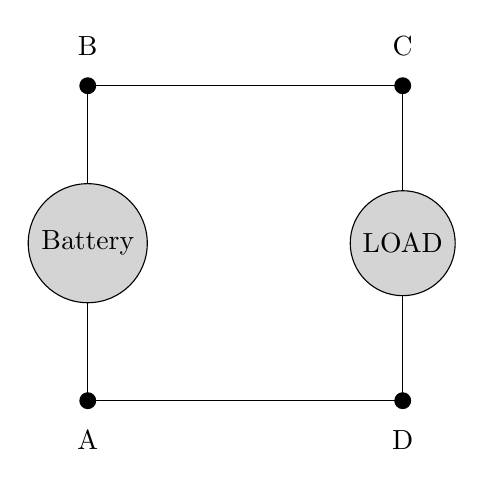
\begin{tikzpicture}
\draw (0,0)--(0,2) node[circle, draw=black,radius=0.25cm, fill={rgb:black,1;white,5}] {Battery}
--(0,4)--(4,4)--(4,2) node[circle, draw=black,radius=0.25cm, fill={rgb:black,1;white,5}] {LOAD}
--(4,0)--cycle;
\filldraw (4,0) circle[radius=1 mm]; \draw node at (4,-.5) {D};
\filldraw (4,4) circle[radius=1 mm]; \draw node at (4,4.5) {C};
\filldraw (0,4) circle[radius=1 mm]; \draw node at (0,4.5) {B};
\filldraw (0,0) circle[radius=1 mm]; \draw node at (0,-.5) {A};
\end{tikzpicture}
\label{F:2BL}
\end{center}
\end{figure}

For example, the network edge from B to C as drawn in Figure~\ref{F:2BL} represents a perfect wire because it was drawn as a line.
\par
\noindent
\begin{itemize}
\item \textbf{Observation:} If a perfect wire connects two nodes, these nodes will be at the same potential (voltage) and behave as one big node.\footnote{You can always decide that a some collection of nodes will be treated as one big node (sometimes called a supernode).} 
\item \textbf{Observation:} The length of a perfect wire does not matter. We'll usually draw whichever length makes the diagram most readable.
\item \textbf{Observation:} When wires cross, a dot indicates a connection.
\end{itemize}
%%%%%%%%%%%%%%%%%%%%%%%%%%%%%%%%%%%%%%%%%%%%%%%%%%%%%%%%%%%%%%%%%%%
\subsection{Switches}
A perfect switch provides a break in the wire when \emph{open} and acts as a perfect wire when \emph{closed}. Figure~\ref{F:2BLa} shows a battery connected to a load via a switch.

\begin{figure}[H]
\begin{center}
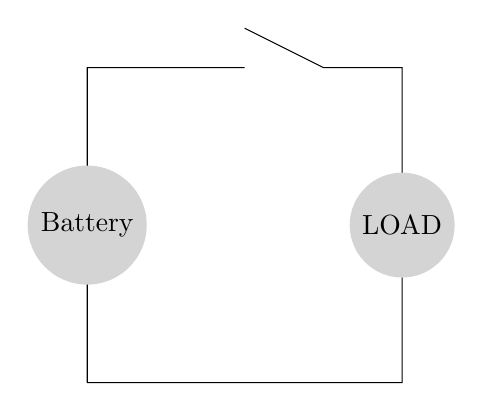
\begin{tikzpicture}
\draw (0,0) node(A){}
--(0,2) node[circle, radius=0.25cm, fill={rgb:black,1;white,5}] {Battery}
--(0,4)--(2,4) (2,4.5)--(3,4)--(4,4)
--(4,2) node[circle, radius=0.25cm, fill={rgb:black,1;white,5}] {LOAD}
--(4,0)
--(0,0);
\end{tikzpicture}
\caption{Battery connected to a load}
\label{F:2BLa}
\end{center}
\end{figure}

When the switch is open, the circuit has three nodes, labeled A, B and C as shown in Figure~\ref{F:2BLb}:

\begin{figure}[H]
\begin{center}
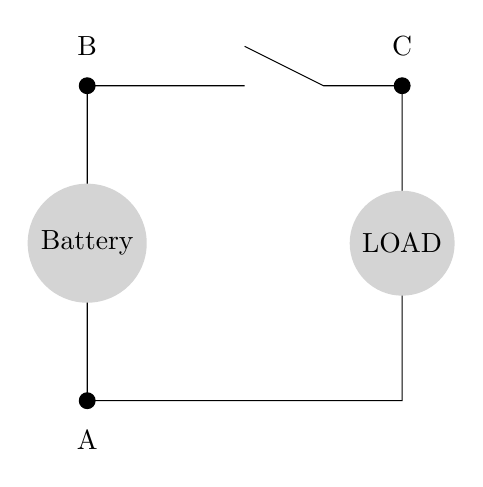
\begin{tikzpicture}
\draw (0,0) node(A){}
--(0,2) node[circle, radius=0.25cm, fill={rgb:black,1;white,5}] {Battery}
--(0,4)--(2,4) (2,4.5)--(3,4)--(4,4)
--(4,2) node[circle, radius=0.25cm, fill={rgb:black,1;white,5}] {LOAD}
--(4,0)--(0,0);
\filldraw (0,0) circle[radius=1 mm]; \draw node at (0,-.5) {A};
\filldraw (0,4) circle[radius=1 mm]; \draw node at (0,4.5) {B};
\filldraw (4,4) circle[radius=1 mm]; \draw node at (4,4.5) {C};
\end{tikzpicture}
\caption{Battery connected to a load with nodes indicated.}
\label{F:2BLb}
\end{center}
\end{figure}

When the switch is closed, the network has only two nodes. Nodes B and C become the same node, because they are connected with a perfect wire.\\
\linebreak
Many homes have three-way switches. The national electric code requires them for some situations like stairwells. With a three-way switch, one can turn off the stairwell light from the top or bottom of the staircase.
\par
Figure~\ref{F:23W} shows how such a switch might operate. The blue wire is the ground wire. We'll discuss that wire and its purpose later.
\par
\begin{figure}[H]
\begin{center}
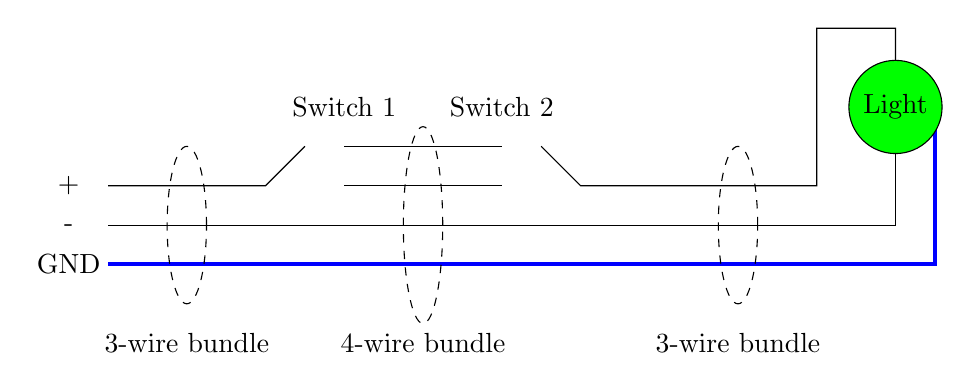
\begin{tikzpicture}
\draw [draw=blue, line width=0.5mm] (0,0) --(10.5,0)--(10.5,2) node(A){};
\draw (0,.5)--(10,0.5)--(10,2);
\draw (0,1)--(2,1)--(2.5,1.5);
\draw (3,1.5)--(5,1.5);
\draw (3,1)--(5,1);
\draw (5.5,1.5)--(6,1)--(9,1)--(9,3)--(10,3)--(10,2) node[circle,radius=.5cm,fill=green,draw=black](L) {Light};
\node at (3,2) {Switch 1};
\node at (5,2) {Switch 2};
\node at (1,-1) {3-wire bundle};
\node at (4,-1) {4-wire bundle};
\node at (8,-1) {3-wire bundle};
\draw [dashed] (1,.5) ellipse (.25 cm and 1 cm);
\draw [dashed] (4,.5) ellipse (.25 cm and 1.25 cm);
\draw [dashed] (8,.5) ellipse (.25 cm and 1 cm);
\node at (-.5,1) {+};
\node at (-.5,.5) {-};
\node at (-.5,0) {GND};
\end{tikzpicture}
\caption{Diagram showing a possible connection for a three-way switch. Note that a special wire with four leads is needed between the two switches.}
\label{F:23W}
\end{center}
\end{figure}

\begin{clevel}
Someone wants to wire a light where any of 3 switches can turn it on or off. Draw an appropriate sketch to show how that might be done. Include the ground wire in your sketch. Hint: You might need to invent another type of switch called a 4-way switch.
\end{clevel}

%%%%%%%%%%%%%%%%%%%%%%%%%%%%%%%%%%%%%%%%%%%%%%%%%%%%%%%%%%%%%%%%%%%%%%
\subsection{The Third Prong}
A plug designed for a wall outlet has three prongs. It is easy to imagine why we need two of them, but what is the purpose of the third prong? After all, some electrical products only have two prongs.\par

If one were to measure the voltages at each prong compared to GND, one of the prongs would read 120 V while the other two would both read zero\footnote{This is 120 VAC rms. We'll get to this later.}. Why do we need the third wire?\par

The reason involves safety. High voltages (like 120V) are dangerous. Consider the electric light shown in this diagram:

\par
\begin{figure}[H]
\begin{center}
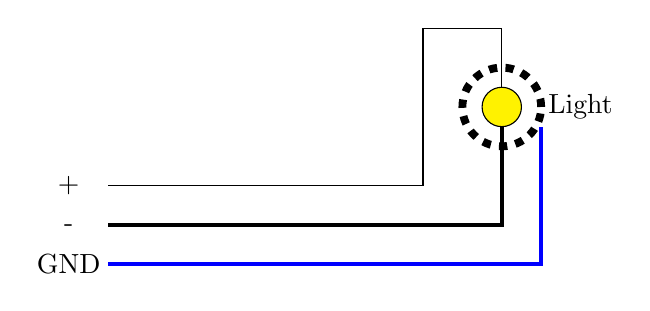
\begin{tikzpicture}
\draw [draw=blue, line width=0.5mm] (0,0) --(5.5,0)--(5.5,1.75) node(A){};
\draw [draw=black, line width=0.5mm] (0,.5)--(5,0.5)--(5,1.75);
\draw (0,1)--(4,1)--(4,3)--(5,3);
% (5,2); node[circle,radius=1cm,draw=black, line width=0.5 mm](L) {Light};
\draw (5,3)--(5,2.25);
\node[draw,circle,minimum size =0.5cm, fill=yellow] at (5,2){};
\node[draw,circle,minimum size =1cm, line width=1 mm, dashed] at (5,2){};
\node at (-.5,1) {+};
\node at (-.5,.5) {-};
\node at (-.5,0) {GND};
\node at (6,2) {Light};
\end{tikzpicture}
\caption{Light fixture showing ground wire protection. The dashed line represents the fixture's metal casing.}
\label{F:23P}
\end{center}
\end{figure}

Consider the situations shown in Table~\ref{T:2P3}:\par
\begin{table}[H]
\begin{center}
\begin{tabular}{c|c|c|c}
two prong or three prong?&status&person touching casing&shock hazard?\\ \hline
2	&	no problem	& yes	& no\\ \hline
2	&	case 1		& no	& no\\ \hline
2	&	case 1		& yes	& \textbf{yes}\\ \hline
2	&	case 2		& yes	& no\\ \hline
3	&	no problem	& yes	& no\\ \hline
3	&	case 1		& no	& no\\ \hline
3	&	case 1		& yes	& no*\\ \hline
3	&	case 2		& yes	& no\\ \hline
\end{tabular}\par
\caption{Situations with 2-prong or 3-prong wiring}
\label{T:2P3}
\end{center}
\end{table}

\begin{itemize}
\item Case 1. The + and nuetral (-) wires have rusted and broken off the light. The +wire touches the light casing.
\item Case 2. The + and neutral (-) wires have rusted and broken off the light. The neutral (-) touches the light casing.
\end{itemize}

Consider case 1 with the + wire contacting the casing. If the casing is grounded via the extra wire (connected to the third prong), then as soon as the + wire comes into contact with the casing, a large current will flow from the + wire through the casing, through the third wire and back to the breaker box. This current will likely exceed the 10 or 15A limit for the circuit breaker. This current will trip the breaker and shut off the circuit. By the time a person unwittingly touches the casing, the circuit should be disconnected and the person should be OK.\par

Of course, the light will no longer work and someone might notice. When the person tries to reset the breaker, the breaker should immediately re-trip, indicating a problem and maybe a hazard.\par

\begin{blevel}
Draw a sketch like Figure~\ref{F:23P}, but for the situation occuring in row 7 of the table.
\end{blevel}
%%%%%%%%%%%%%%%%%%%%%%%%%%%%%%%%%%%%%%%%%%%%%%%%%%%%%%%%%%%%%%%%%%%%%%%
\subsection{Light-bulbs}
A light-bulb or LED is a device that converts electrical energy into photons that are visible to the human eye. Older incandescent light bulbs operate by making a wire so hot that it glows white. This type of bulb wastes most of the energy as heat. Think of it like using a campfire to light up a living room.
Newer bulbs, like LEDs, more directly create photons and are much more efficient.

\begin{alevel}
What does LED stand for?
\end{alevel}

\begin{blevel}
What is a diode?
\end{blevel}

\begin{alevel}
At what temperature must something be in order to glow red? Look it up online.
\end{alevel}

\subsection{Voltage sources}
A voltage source produces a constant voltage difference between two points, almost regardless of the amount of current that would be needed.
\par
Solar panels represent decent voltage sources because they produces roughly steady voltages. More sunlight allows the panel to provide more current and therefore more power, but the voltage remains roughly the same.
\par
A wall socket also represents a fairly ideal voltage source, at least until the current exceeds the limit for the circuit breaker at which point the voltage goes to zero. Wall sockets in the US produce about 120 Volts AC, and provide roughly the same voltage difference whether you draw 1 Amp of current or 10 Amps of current. 

\par
\subsection{Current sources}
Current sources provide steady currents instead of steady voltages. The symbols for voltage sources and current sources are shown in Figure~\ref{F:2SCV}.
\par

\begin{figure}[H]
\begin{center}
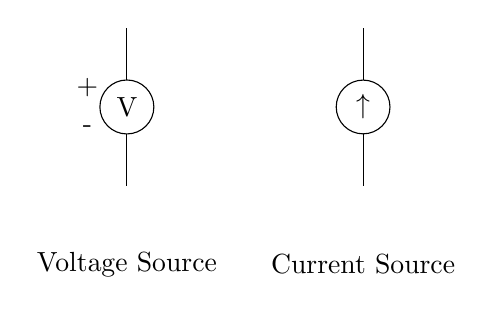
\begin{tikzpicture}
\node at (1,-1) {Voltage Source};
\node at (4,-1) {Current Source};
\draw (1,0)--(1,1) node[circle, draw=black, radius=1cm, fill=white]{V}--(1,2);
\node at (0.5,1.25) {+};
\node at (0.5,.75) {-};
\draw (4,0)--(4,1) node[circle, draw=black, radius=2cm, fill=white]{$\uparrow$}--(4,2);
\end{tikzpicture}
\caption{Symbols for voltage sources and current sources.}
\label{F:2SCV}
\end{center}
\end{figure}

Note the plus-minus indication on the voltage source. This indicates which side is more positive. The current source arrow already shows the direction of the current. If the current source were negative, then the current flows opposite the direction of the arrow.

\subsection{Resistors}
Unlike perfect wires, resistors are so named because they hinder or \emph{resist} the flow of current. It takes effort (energy) to push charge through a resistor. The more charge per second you need to get through the resistor, the more energy (effort) it will take.
\par
\begin{alevel}
What is another name for energy per charge?
\end{alevel}

For some objects, like a typical chunk of metal, the flow (current) varies roughly proportionally to the change in the voltage across it. This is captured by something called Ohm's Law.
\par
\begin{align*}
\Delta V \sim I	&&\text{Ohm's Law}
\end{align*}

The proportionality constant can be written as R.\par
\begin{align}
\Delta V = IR	&&\text{Ohm's Law}
\end{align}
 Note: the $\Delta$ on the $\Delta V$ is often omitted because it is usually obvious that you're referring to a change in voltage, and not some meaningless absolute voltage with respect to who-knows-what reference point. \par

\begin{alevel}
What is the standard S.I. unit of resistance?
\end{alevel}

\begin{clevel}
In terms of Coulombs, seconds, and Joules, what are the units of resistance?
\end{clevel}

\begin{clevel}
In terms of Coulombs, seconds, meters, and kg, what are the units of resistance? Hint: What is a Joule?
\end{clevel}

For better or worse, Ohm's law is NOT some fundamental relationship that is true all the time. Instead, it is only sort-of true some of the time. Manufactured resistors, like the ones in the lab, are designed mimic Ohm's Law pretty well. Other devices, like LEDs, do not much behave this way at all.\par

\begin{blevel}
Which of the following formulae are perfectly accurate (either because its a definition or because it is a model that has not (yet) been contradicted by experiment) verses a approximate model (hack) that we know is not exactly right?\\
\begin{center}
\begin{tabular}{|c|c|}\hline
equation & (always correct) or (hack)? \\ \hline
$F_f=\mu F_N$ & \\ \hline
$V=IR$ & \\ \hline
$\rho=\frac{mass}{Vol}$ & \\ \hline
$PV=nRT$ & \\ \hline
\end{tabular}
\end{center}
\end{blevel}

Resistors on a diagram are drawn with a zig-zag line. Figure~\ref{F:21} shows a current source connected to a $5 \Omega$ resistor.

\begin{figure}[H]
\begin{center}
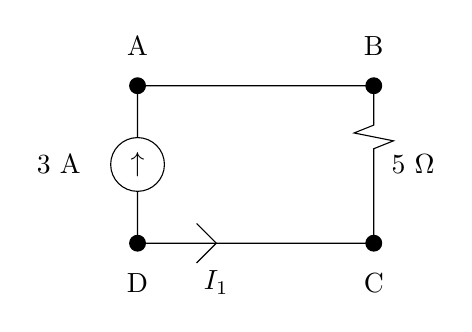
\begin{tikzpicture}
\draw (1,0)--(1,1) node[circle, draw=black, radius=2cm, fill=white]{$\uparrow$}--(1,2)--(4,2)--(4,1.5)--(3.75,1.4)--(4.25,1.3)--(4,1.2)--(4,0)--(1,0);
\node at (0,1) {3 A};
\node at (4.5,1) {5 $\Omega$};
\filldraw (1,2) circle[radius=1 mm];
\node at (1,2.5) {A};
\filldraw (4,2) circle[radius=1 mm];
\node at (4,2.5) {B};
\filldraw (4,0) circle[radius=1 mm];
\node at (4,-.5) {C};
\filldraw (1,0) circle[radius=1 mm];
\node at (1,-.5) {D};
\draw (1.75,.25)--(2,0)--(1.75,-.25);
\node at (2,-.5) {$I_1$};
\end{tikzpicture}
\caption{A current source connected to a resistor. Note how current $I_1$ is labeled with an arrow.}
\label{F:21}
\end{center}
\end{figure}

\begin{blevel}
Fill in Table~\ref{T:21}.
\end{blevel}

\begin{table}[H]
\begin{center}
\begin{tabular}{|c|c|c|}\hline
item&answer&hints\\ \hline
$I_1$	&	&	\\ \hline
$V_{AB}$	&	&	\\ \hline
$V_{BC}$	&	& use Ohm's law	\\ \hline
$V_{AD}$	&	&	\\ \hline
$I_{from B to C}$	&	&	\\ \hline
Power absorbed by R	&	&	\\ \hline
Power produced by current source	&	&	\\ \hline
\end{tabular}
\label{T:21}
\caption{Summary of select parameters for simple circuit.}
\end{center}
\end{table}

One can connect resistance (an extrinsic property) to resistivity (an intrinsic property). \footnote{An \textbf{extrinsic} property depends on something's amount or shape. An \textbf{intrinsic} property does not depend on how much of it you have. Density is an intrinsic property whereas mass is not.}\par

\begin{align}
R = \rho \frac{L}{A} \label{E:2rho}
\end{align}
Where $\rho$ is the resistivity of the material, L is its length and A is its cross-sectional area.

\begin{blevel}
Determine the resistance of a 20 m long section of 12 gauge copper wire. Hint: look up the radius of 12 gauge wire. 12-gauge wire is typical for household wiring.
\end{blevel}

\begin{blevel}
An aluminum wire inside a computer chip carries a signal from one side of the chip to the other. The dimensions of the wire are 5 mm by 1 micron by 0.1 micron. What is the resistance of the wire? If 100mA of current pass through the wire, what is the voltage dropped across it? How much power is dissipated by the wire? 
\end{blevel}

\begin{dlevel}
Continuing the previous problem. If the heat had nowhere to go but to heat up the Al wire, how much would the temperature of the wire increase after 1 minute? How much time until the wire melted?
\end{dlevel}

We can substitute Equation~\eqref{E:2rho} expression for resistance into Ohm's law and come up with an equation for electricity flow that is very similar to the flow of heat.

\begin{align*}
I = \frac{\Delta V}{R}	\\
\frac{dq}{dt} = \frac{\Delta V}{\rho}\frac{A}{L}=(\frac{1}{\rho})\frac{A\Delta V}{L}&&	\text{``electricity flow" equation}\\
\frac{dQ}{dt}=	\frac{kA\Delta T}{L}&&				\text{heat flow equation}
\end{align*}
What drives heat to flow from one side of a material to the other? Answer: a temperature difference. What drives electrical charge to flow from one side of a material to the other? Answer: a voltage difference.

\begin{blevel}
A 0.5 meter long section of 12-gauge Cu wire connects between the inside of a house ($65^0 F$) and the outside of a house ($35^0 F$). How many Joules of heat flow out of the house through the wire in one minute?
\end{blevel}

\begin{blevel}
A 0.5 meter long section of 12-gauge Cu wire connects between one side of a 9V battery and the other. How many Coulombs of charge flow along the wire in one minute?
\end{blevel}

